%!TEX program = xelatex
%%%%%%%%%%%%%%%%%%%%%%%这是导言部分的开始%%%%%%%%

%========= 导言部分声明文档的类型=================
\documentclass{article}

%=========导言部分可可以加载宏包=================
\usepackage{amsmath}                % 数学公式排版宏包
\usepackage{amssymb}                % 数学符号命令宏包
\usepackage{amsthm}                 % 数学定理宏包
\usepackage[UTF8]{ctex}             % 中文输入宏包
\usepackage[a4paper]{geometry}      % 页面设置宏包
\usepackage{setspace}               % 行间距宏包
\usepackage{graphicx}               % 图片宏包
\usepackage{listings}               % 代码宏包
\usepackage{color}					% 颜色宏包
\usepackage{xcolor}                 % 颜色处理宏包
\usepackage{float}                  % 浮动对象式样宏包
\usepackage{fontspec}
\usepackage{enumerate}				% 列举编号包

%=========页面设置==============================
\geometry{left=1cm,right=1cm,top=1cm,bottom=2cm}
\onehalfspacing
\setlength\parindent{0em}

%=========代码格式设置============================
\definecolor{dkgreen}{rgb}{0,0.6,0}
\definecolor{gray}{rgb}{0.5,0.5,0.5}
\definecolor{mauve}{rgb}{0.58,0,0.82}
% \setmonofont{Consolas}
\lstset{
	numbers = left, 	
	numberstyle = \color{gray}, 
	keywordstyle = \color{blue},
	commentstyle = \color{dkgreen}, 
	stringstyle = \color{mauve},
	basicstyle = \ttfamily,
	breaklines = true,
	frame = shadowbox, % 阴影效果
	rulesepcolor = \color{ red!20!green!20!blue!20} ,
	escapeinside = ``, % 英文分号中可写入中文
	xleftmargin = 2em,xrightmargin=2em, aboveskip=1em,
	framexleftmargin = 2em
} 

%=========导言部分可以定义标题信息===============
\title{组会报告}
\author{徐益}
\date{\today}
%%%%%%%%%%%%%%%%%%%%%%%这是导言部分的结束%%%%%%%%%

%%%%%%%%%%%%%%%%%%%%%%%这是正文部分的开始%%%%%%%%%
\begin{document}

%=========生成标题================================
\maketitle

%=========开始正文的输入==========================

%===========第一节=================
\section{工作内容} 
1. 处理1200子载波下的导频问题;

2. 生成1344子载波下的模拟信道;

3. 实现新的单线程系统。

%===========第二节=================
\section{处理1200子载波下的导频问题}
\subsection{问题}
\begin{figure}[H]
	\centering
	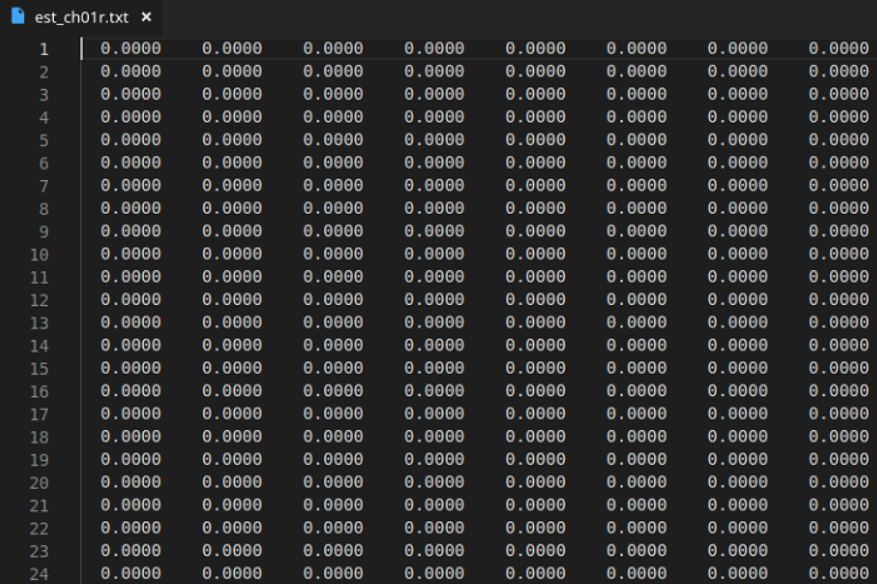
\includegraphics[width = .8\textwidth]{errch.png}
	\caption{信道估计错误}
\end{figure}
\begin{figure}[H]
	\centering
	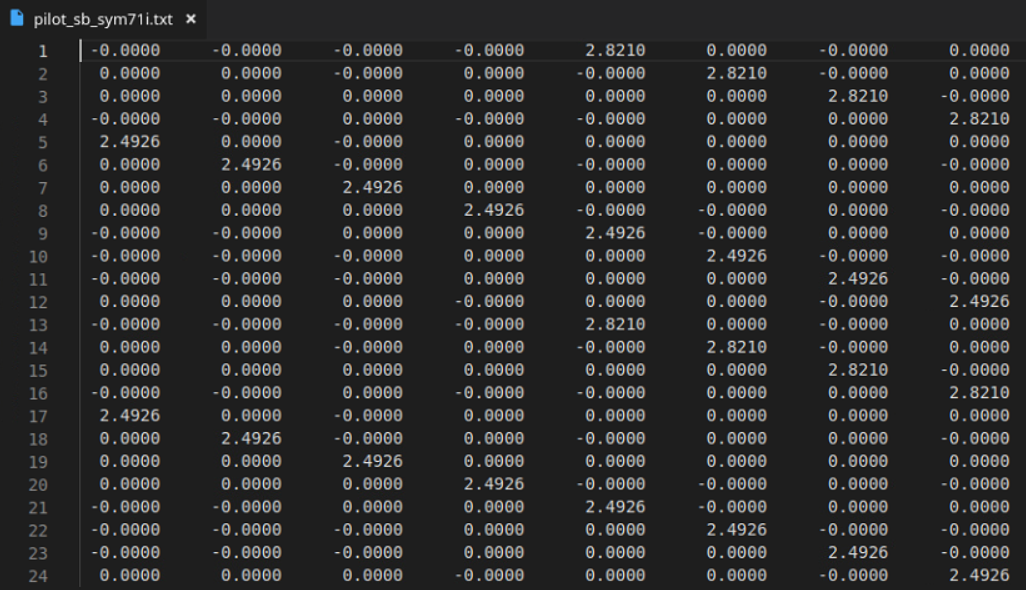
\includegraphics[width = .8\textwidth]{errpilot.png}
	\caption{每个资源块的导频序列问题}
\end{figure}
\subsection{解决}
选择1344(4*336)子载波

%===========第三节=================
\section{生成1344子载波下的模拟信道}
\subsection{SCM信道生成失败}
\begin{figure}[H]
	\centering
	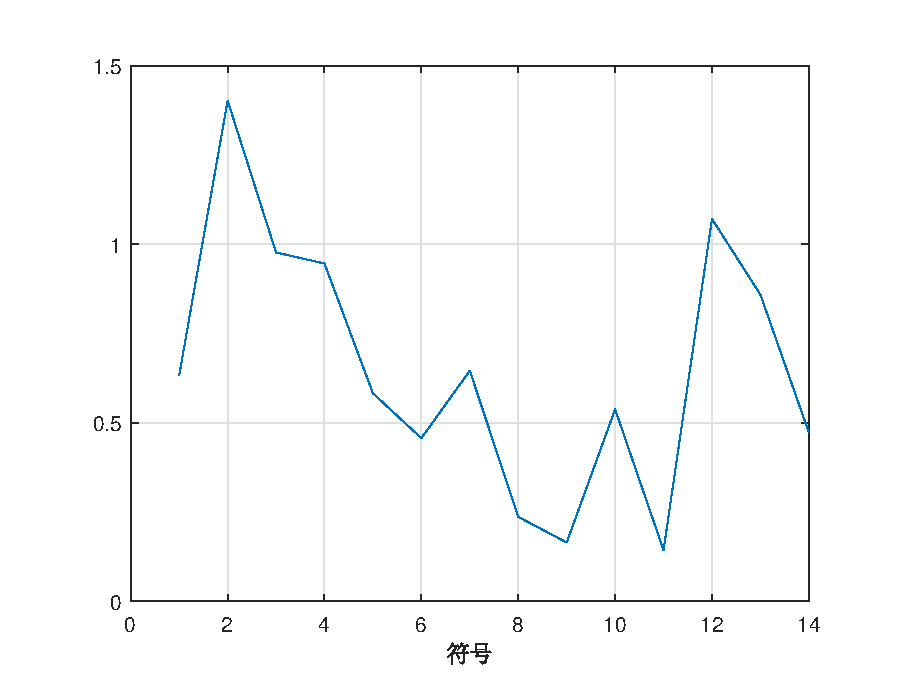
\includegraphics[width = .7\textwidth]{old.eps}
	\caption{生成的SCM信道时间方向上的性能}
\end{figure}
\subsection{WinnerII信道生成}
\begin{figure}[H]
	\centering
	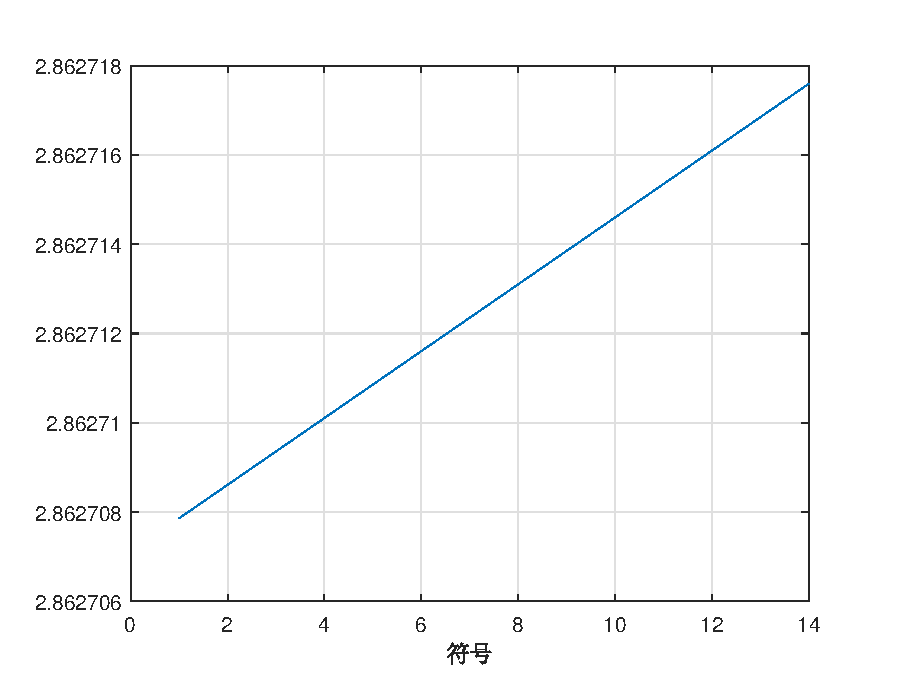
\includegraphics[width = .7\textwidth]{new.eps}
	\caption{生成WinnerII信道时间方向上的性能}
\end{figure}
\begin{figure}[H]
	\centering
	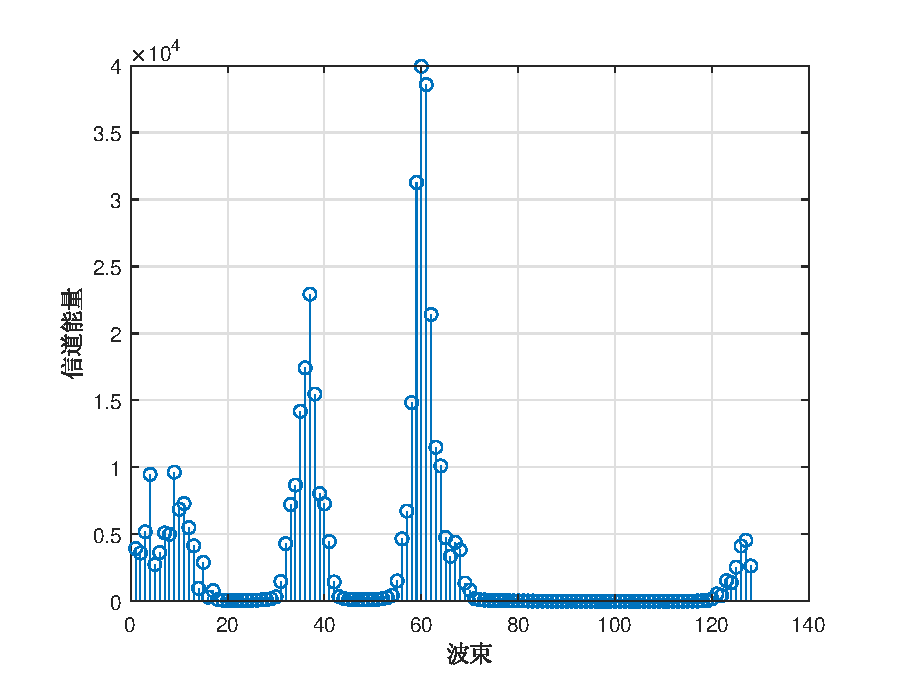
\includegraphics[width = .7\textwidth]{power.eps}
	\caption{波束域信道能量分布}
\end{figure}

%===========第四节=================
\section{实现新的单线程系统}
\begin{figure}[H]
	\centering
	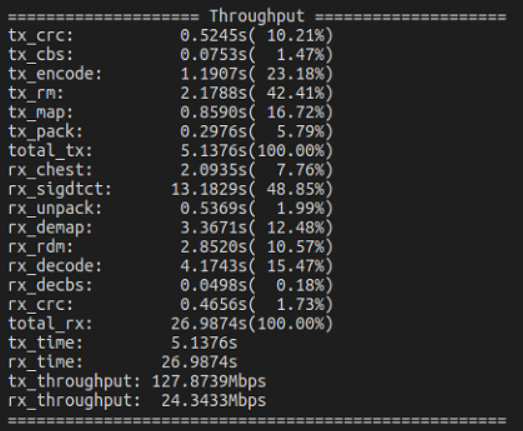
\includegraphics[width = .6\textwidth]{res.png}
	\caption{性能测试结果}
\end{figure}
$tx_{part1} = 0.0391ms(\times 8VTB\times 11CB)$\\
$tx_{part2} = 0.1446ms(\times 8VTB)$\\
$rx_{part1} = 0.2824ms(\times 4VTB\times 14SB)$\\
$rx_{part2} = 0.1187ms(\times 8VTB\times 11CB)$

%===========第五节=================
% \section{有PRACH情况下的资源分配问题}
% \begin{figure}[H]
% 	\centering
% 	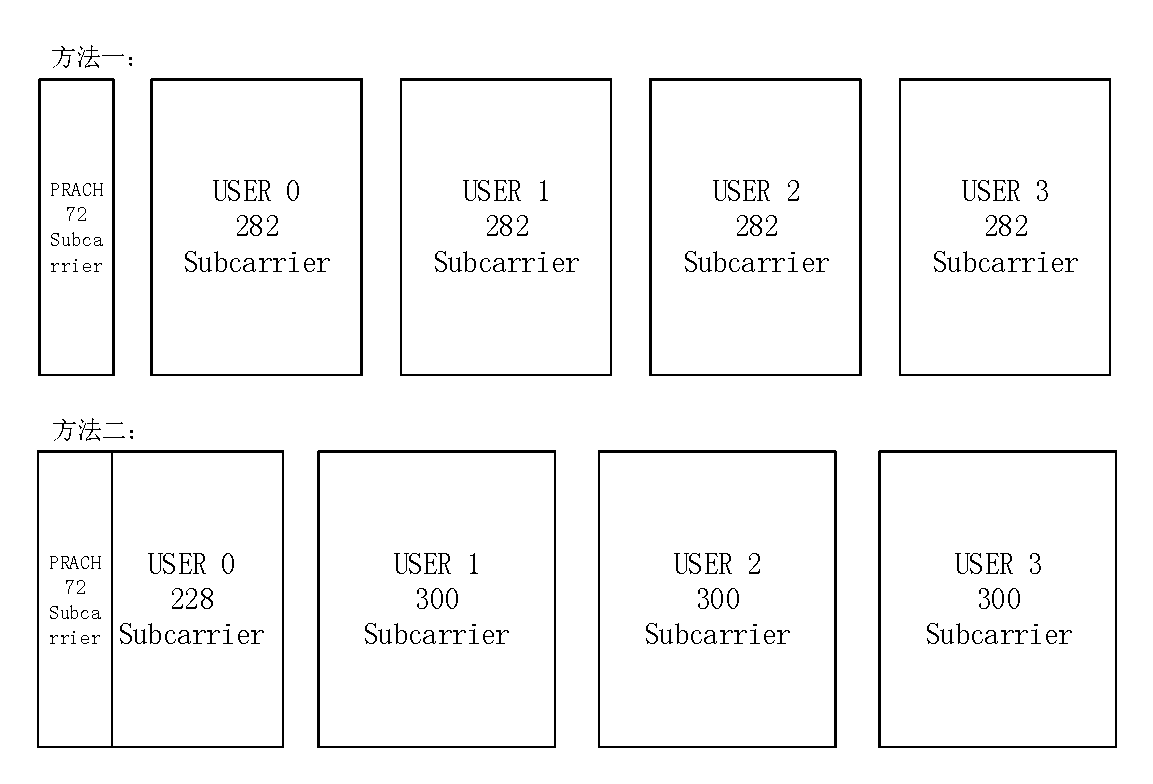
\includegraphics[width = \textwidth]{ques.pdf}
% 	\caption{两种方案}
% \end{figure}

%===========下周计划=================
% \section{下阶段计划}
% 1. 完善单线程系统(修复Bug)

\end{document}
%%%%%%%%%%%%%%%%%%%%%%%这是正文部分的结束%%%%%%%%%%%%